% This is samplepaper.tex, a sample chapter demonstrating the
% LLNCS macro package for Springer Computer Science proceedings;
% Version 2.21 of 2022/01/12
%
\documentclass[runningheads]{llncs}
%
\usepackage[T1]{fontenc}
% T1 fonts will be used to generate the final print and online PDFs,
% so please use T1 fonts in your manuscript whenever possible.
% Other font encondings may result in incorrect characters.
%
\usepackage{graphicx}
\usepackage{placeins}
% Used for displaying a sample figure. If possible, figure files should
% be included in EPS format.
%
% If you use the hyperref package, please uncomment the following two lines
% to display URLs in blue roman font according to Springer's eBook style:
%\usepackage{color}
%\renewcommand\UrlFont{\color{blue}\rmfamily}
%\urlstyle{rm}
%
\begin{document}
%
\title{CRAFT: Exploiting Precharge Cost Asymmetry for Adaptive DRAM Row Buffer Management}
%
\titlerunning{CRAFT: Adaptive DRAM Row Buffer Management}
%
\author{First Author\inst{1}\orcidID{0000-1111-2222-3333} \and
Second Author\inst{2,3}\orcidID{1111-2222-3333-4444} \and
Third Author\inst{3}\orcidID{2222--3333-4444-5555}}
%
\authorrunning{F. Author et al.}
% First names are abbreviated in the running head.
% If there are more than two authors, 'et al.' is used.
%
\institute{Princeton University, Princeton NJ 08544, USA \and
Springer Heidelberg, Tiergartenstr. 17, 69121 Heidelberg, Germany
\email{lncs@springer.com}\\
\url{http://www.springer.com/gp/computer-science/lncs} \and
ABC Institute, Rupert-Karls-University Heidelberg, Heidelberg, Germany\\
\email{\{abc,lncs\}@uni-heidelberg.de}}
%
\maketitle              % typeset the header of the contribution
%
\begin{abstract}
DRAM row buffer management presents a fundamental tradeoff between exploiting row buffer locality and minimizing conflict penalties. The optimal policy varies across workloads, execution phases, and individual address ranges. Existing adaptive schemes, however, face a persistent tension between hardware complexity and management effectiveness.

This paper presents CRAFT (Cost-driven Row-buffer Adaptive Feedback Timeout), a lightweight, feedback-driven row buffer management scheme. CRAFT exploits a fundamental cost asymmetry in timeout-based speculative precharge. The purpose of speculative precharge is to preserve row buffer locality while selectively closing idle rows. Both the precharge and the subsequent reactivation induced by a wrong precharge are entirely unnecessary and would not occur under the open-page scenario. A conflict, where the next access targets a different row, carries a fundamentally different cost. The precharge and activation are inherent to the access pattern regardless of the timeout decision, and only the opportunity to overlap precharge with idle bank cycles is lost. CRAFT translates this asymmetry into differentiated per-bank timeout adjustments. Wrong precharges escalate the timeout through exponential backoff, and conflicts de-escalate it with a smaller step proportional to the avoidable overhead. Beyond this core feedback loop, three precharge-path refinements further improve adaptation precision without additional hardware structures. The entire mechanism requires no prediction tables, feature extraction, or learned models.

We evaluate CRAFT using a cycle-accurate simulator across 12 memory-intensive workloads from graph analytics and scientific computing. CRAFT achieves geometric mean IPC improvements of 7.73\%, 3.10\%, and 2.84\% over ABP, DYMPL, and INTAP, respectively, consistently outperforming all evaluated baselines. The total storage overhead is 140~bytes per channel, representing a 24$\times$ reduction relative to DYMPL and over 140$\times$ reduction relative to ABP. These results demonstrate that the cost asymmetry inherent in precharge outcomes provides a sufficient and lightweight foundation for effective row buffer management.

\keywords{DRAM row buffer management \and page policy \and memory controller \and feedback-driven adaptation}
\end{abstract}
%
%
%
\section{Introduction}

Main memory latency remains a primary performance bottleneck in modern processor systems~\cite{Wulf95,Mutlu13,Hennessy19}.
A critical factor governing this latency is how the memory controller manages the \emph{row buffer} in each DRAM bank, the internal sense-amplifier array that caches the most recently activated row.
Holding a row open (the \emph{open-page} policy) maximizes the chance of serving subsequent accesses to the same row at low latency, but risks expensive conflicts when a different row is potentially needed. Closing immediately after each access (the \emph{close-page} policy) eliminates such conflicts but forfeits all potential row locality.
This fundamental tradeoff makes row buffer management one of the most extensively studied yet persistently challenging aspects of memory controller design~\cite{Zhang00,Jacob07}.

The optimal page policy varies across workloads, across execution phases, and even across targeted address ranges.
Neither open-page nor close-page dominates across all workloads. Open-page loses up to 11\% IPC on workloads with frequent row buffer conflicts. Close-page sacrifices up to 28\% IPC on workloads with high row buffer locality (Fig.~\ref{fig:motivation}(a)).
Within a single program execution, row buffer hit rate shifts dramatically between program phases. The row buffer hit rate of \texttt{mcf} transitions from above 90\% hit rate to below 10\%, while \texttt{PageRank} follows the inverse trajectory (Fig.~\ref{fig:motivation}(b)).
Beyond temporal variation, row buffer locality also differs substantially across banks within a single channel. Under the open-page policy, \texttt{omnetpp} exhibits a per-bank row buffer hit rate coefficient of variation of 1.51, indicating pronounced inter-bank disparity.
These observations suggest that effective row buffer management should adapt per bank and per execution phase.

\begin{figure}[!htbp]
\centering
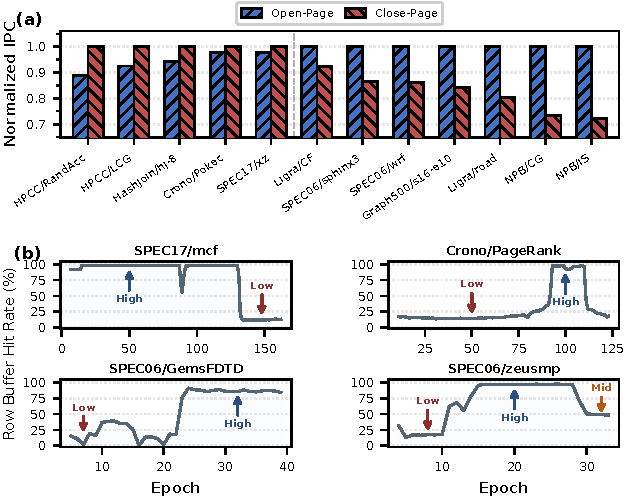
\includegraphics[width=\textwidth]{../figures/output/motivation_combined.pdf}
\caption{(a) Normalized IPC of open-page and close-page policies across 12 memory-intensive workloads, normalized to the better static policy per workload. Neither static policy dominates across all workloads. (b) Row buffer hit rate across execution epochs under the open-page policy for four representative workloads. Each workload exhibits distinct phase transitions between high- and low-locality regimes.}
\label{fig:motivation}
\end{figure}

Achieving per-bank, phase-adaptive row buffer management with low hardware overhead remains an open problem. Prior adaptive schemes have addressed aspects of this challenge but face a fundamental tradeoff between hardware complexity and adaptation precision.
ABP~\cite{Awasthi11} requires approximately 20~KB per channel for per-row prediction tables. DYMPL~\cite{Rafique22} employs a perceptron-based classifier with 3.39~KB per channel and requires machine-learning inference on the critical path. INTAP~\cite{Intel06} adjusts a per-bank timeout using approximately 200~bytes per channel. It applies the same fixed step size to both wrong precharges and conflicts. This symmetric adjustment does not distinguish between the penalty induced by speculative precharge decisions and the inherent cost of the access pattern of the memory request streams.

This paper presents CRAFT (\textbf{C}ost-driven \textbf{R}ow-buffer \textbf{A}daptive \textbf{F}eedback-driven \textbf{T}imeout), a lightweight, feedback-driven row buffer management scheme. Timeout-based speculative precharge preserves row buffer locality and selectively closes idle rows. CRAFT refines this mechanism by exploiting the observation that the three possible precharge outcomes, namely \emph{right}, \emph{wrong}, and \emph{conflict}, produce qualitatively different types of waste.
A right precharge correctly anticipates the end of row-level locality, and no bandwidth is wasted.
A wrong precharge is the most detrimental outcome. The purpose of speculative precharge is to preserve row buffer locality, yet a wrong precharge eliminates precisely this benefit. The subsequent access targets the same row and would have been served as a row buffer hit had the row remained open. Both the precharge and the reactivation are therefore entirely avoidable operations that would not occur under an open-page policy.
A conflict presents a fundamentally different situation. Because the target row differs from the currently open row, the precharge and activation are inherent to the access pattern. These operations would occur regardless of the timeout decision. The only benefit a well-timed precharge could provide is overlapping the precharge penalty with idle bank cycles.
This asymmetry in failure cost is the foundation of CRAFT's feedback mechanism. A wrong precharge generates entirely avoidable overhead, while a conflict forfeits only a latency-hiding opportunity. CRAFT assigns correspondingly different adjustment magnitudes to each outcome. Wrong precharges escalate the timeout by exponentially increasing steps, guarding aggressively against further premature precharges. Conflicts reduce the timeout by a smaller, fixed step, reflecting the comparatively lower cost of a missed overlap. The resulting mechanism requires no prediction tables, feature extraction, or learned models.
With only 140~bytes of state per channel, CRAFT consistently outperforms all three baselines across 12 memory-intensive workloads.

The contributions of this paper are as follows:

\begin{enumerate}
\item We identify that the three outcomes of timeout-based speculative precharge produce qualitatively different types of waste. A wrong precharge introduces entirely avoidable overhead. A conflict incurs only the inherent cost of the access pattern. We propose CRAFT, a feedback-driven scheme that translates this cost asymmetry into differentiated timeout adjustments per bank. The entire mechanism requires only 140~bytes per channel.
\item Through ablation analysis, we demonstrate that feedback signals derived from precharge outcomes are sufficient for effective timeout adaptation in our evaluated setting, without requiring auxiliary runtime metrics.
\item We further show that incorporating conflict-path heuristics does not improve performance. Phase detection and queue occupancy signals introduce noise into the feedback loop rather than useful adaptation information.
\item We evaluate CRAFT using a cycle-accurate simulator with a DDR5-4800 configuration on 12 memory-intensive workloads including graph analytics and scientific computing. CRAFT consistently outperforms all three baselines with over 140$\times$ storage reduction compared to ABP.
\end{enumerate}

\begin{credits}
\subsubsection{\ackname} A bold run-in heading in small font size at the end of the paper is
used for general acknowledgments, for example: This study was funded
by X (grant number Y).

\subsubsection{\discintname}
It is now necessary to declare any competing interests or to specifically
state that the authors have no competing interests. Please place the
statement with a bold run-in heading in small font size beneath the
(optional) acknowledgments\footnote{If EquinOCS, our proceedings submission
system, is used, then the disclaimer can be provided directly in the system.},
for example: The authors have no competing interests to declare that are
relevant to the content of this article. Or: Author A has received research
grants from Company W. Author B has received a speaker honorarium from
Company X and owns stock in Company Y. Author C is a member of committee Z.
\end{credits}
\FloatBarrier
\bibliographystyle{splncs04}
\bibliography{refs}
\end{document}
